\section{System Overview}

\begin{figure*}[t]
		\centering
		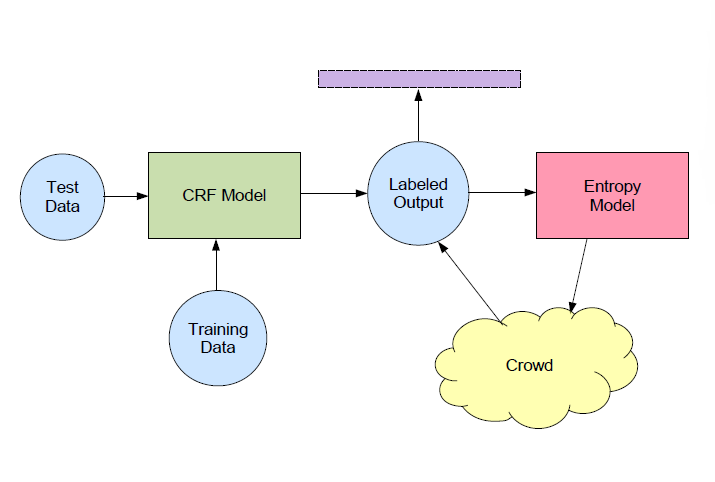
\includegraphics[width=.65\textwidth]{images/system_design.png}
		\label{fig:system}
		\caption{Architecture of the \sysName system.} 
\end{figure*}

This section describes the basic setup of the system.  We extend the in-database CRF model of Wang et al.\cite{DBLP:journals/pvldb/WangFGH10}, giving an overview of the original data model and then discussing our extensions to handle crowd-inserted data and newly inferred evidence.  Afterwards we explore the various operators used to manipulate the data and perform functions such as selecting uncertain tokens, pushing to the crowd, aggregating the result, and integrating new evidence into the final query results. 

\subsection{Data Model}

We treat unstructured text as consisting of a set of documents or text-strings $\mathcal{D}$.  Each document $d\in\mathcal{D}$ has substructure comprising a set of tokens $t^{d}_{i}$, where $i\in\left\{1,...,N\right\}$ and $N$ is the length of the string.  Specific documents $d$ are identified  by a unique identifier (docID) and tokens $t^{d}_{i}$ are identified by their associated docID and their position $i$ within $d$.

T{\small OKEN}T{\small BL} and F{\small ACTOR}T{\small BL} below are identical to the versions found in \cite{DBLP:journals/pvldb/WangFGH10}.  In order to provide an interface for human-corrected answers we introduce C{\small ROWD}P{\small OST}T{\small BL} for keeping track of questions posted to the crowd, C{\small ROWD}A{\small NS}T{\small BL} for storing responses, and E{\small VIDENCE}T{\small BL} comprising aggregated evidence used to constrain the inference process at query time.

\noindent\textbf{Token Table:} The token table T{\small OKEN}T{\small BL} is an incomplete relation $R$ in $\mathcal{DB^{P}}$, which stores text-strings as relations in \sysName .  The structure is similar to that found in inverted file systems commonly used in information retrieval.  As previously mentioned the primary key for each token is the docID and position (pos) attributes.  The token also contains one probabilistic attribute\textemdash label$^{p}$.  Its values are left initially empty and are inferred from a combination of the learned machine model and crowd-provided labels.

\vspace{.1in}
\centerline{T{\small OKEN}T{\small BL}(docID, pos, token, label$^{p}$)}
\vspace{.1in}

\noindent\textbf{Factor Table:} The F{\small ACTOR}T{\small BL} allows for a direct computation of the possible "worlds" of T{\small OKEN}T{\small BL} from within \sysName according to the CRF model.  It is a materialization of the \emph{factors} used to calculate edge potentials $\varphi[y_{i},y_{i-1}|x_{i-1}]$ to determine the most likely labeling of the tokens in corpus $\mathcal{D}$.  In the CRF model, these factors defining the correlation between $x_{i}$, $y_{i}$, and $y_{i-1}$ are the weighted sum of feature functions: $\varphi[y_{i},y_{i-1}|x_{i}] = \sum^{K}_{k=1}\lambda_{k}f_{k}(y_{i},y_{i-1},x_{i})$.

These features are typically binary and denote the presence or absence of $x_{i}$, $y_{i}$, and $y_{i-1}$ appearing together in the model.  The weights are learned from training and provide a score to the set of correlated variables.  F{\small ACTOR}T{\small BL} contains each triple along with its associated score.

\vspace{.1in}
\centerline{F{\small ACTOR}T{\small BL}(token, prevLabel, label, score)}
\vspace{.1in}

\noindent\textbf{Crowd Post Table:} The set of tokens $\mathcal{T}$ that are selected to be hand-labeled need a means of mapping to and from the Amazon Mechanical Turk service.  Each submitted HIT is given a unique HITID by Amazon, which is stored in C{\small ROWD}P{\small OST}T{\small BL} to maintain token identities upon retrieval for each $t\in\mathcal{T}$.  Since many tokens are mapped into a single HIT, as we describe later in Section ~\ref{hit}, the table also includes the question position (HITpos).
 
\vspace{.1in}
\centerline{C{\small ROWD}P{\small OST}T{\small BL}(docID, pos, HITID, HITpos)}
\vspace{.1in}

\noindent\textbf{Crowd Answer Table:} The crowd's responsibility is to provide labels from the set $\mathcal{L}$ for all tokens pushed to the AMT service.  Individual labels $l\in\mathcal{L}$ retrieved for each HIT are stored in C{\small ROWD}A{\small NS}T{\small BL} along with a set of identifiers for the HIT (HITID \& HITpos) and the Turker herself (workerID).  Performing a JOIN with C{\small ROWD}P{\small OST}T{\small BL} produces a set of token-label pairs.  However, since question redundancy is one method of quality control there may be more than one label per token and the answers must be aggregated before they may be used.  This is discussed more in Section ~\ref{integration}.

\vspace{.1in}
\centerline{C{\small ROWD}A{\small NS}T{\small BL}(HITID, HITpos, workerID, label)}
\vspace{.1in}

\noindent\textbf{Evidence Table:} When the Viterbi process is run, it consults the evidence table E{\small VIDENCE}T{\small BL} and constrains the result accordingly.  It has the same format as T{\small OKEN}T{\small BL}, but while the latter is constructed purely from the extracted ML output, the former is drawn from additional sources and take precedence over the extraction.  The probabilistic attribute, label$^{p}$, represents a probabilistic aggregation of the wisdom of the crowd.  Section ~\ref{integration} contains an explanation of the entire integration process.

\vspace{.1in}
\centerline{E{\small VIDENCE}T{\small BL}(docID, pos, token, label$^{p}$)}
\vspace{.1in}

\subsection{\sysName Operations}

The operations of \sysName are defined over a set of User-Defined Functions (UDF) on the relational tables that express the full fuctionality of the system.  Apart from traditional insert, remove, and query operations, \sysName has a number of more complex functions that update the internal state of the system.  These generally fall into functions supporting one of three broader operations: selection, aggregation, and integration.

Selection of uncertain tokens is based on information theoretic uncertainty sampling.  \sysName has functionality for computing marginal distributions over token labelings and the associated entropy of those distributions.  A question queue is created for pushing tokens to AMT ranked by highest entropy.  System-specific optimizations include clustering over duplicated tokens to prevent redundancy in question submissions and restricting to one token per document $d$.

Aggregation is used as a means of preserving the quality of answers.  The gold standard is to increase the number of workers that answer each question and take a majority vote among their responses.  In our studies we've found that a Bayesian approach based on perceived Turker quality produces consistently better results and has the advantage of being probabilistic.  This technique is implemented in \sysName along with the sub-function to calculate worker quality.

Finally, integration allows the database to use the crowd-aggregated result to improve its own extraction results.  The vanilla Viterbi is replaced by a Constrained Viterbi that modifies its path according to feedback in its evidence table.  The user has the ability to place a threshold on the entropy of probabilistic evidence values to ensure only high quality, trusted feedback is actually used.     

The remainder of this paper will be spent fleshing out the procedures behind selection, aggregation, and integration.  Specific UDFs will be reviewed for each section, while full pseudo-code and SQL statements can be found in the Appendix.






\eat{\sean{Still need to excise and change most of this section in terms of new model and operators.}

\sysName is a system that combines the power of the crowd and machine learning to solve problems in text extraction and labeling.  At its core is a probabilistic database defined as a set of base tables capable storing the uncertainty in the extraction process as well as a set of operators over these tables that perform jobs such as the intial extraction, querying the crowd, and integrating new data from various sources.

Figure ~\ref{fig:system} shows the main architecture of \sysName.  At the base is a set of uncertain tables connected by an underlying probabilistic graphical model interface.  \sean{Read Bayestore to get a better idea of how to describe this PGM model}.
  

\eat{The upper block denotes a number of standard database functions populated by machine learning algorithms.  Initially unstructured text goes through a preprocessing stage where it is tokenized and converted to lower case.  The CRF performs segmentation and labeling adhering to a specified schema and deposits the results into the database along with number of statistical metadata including marginal probabilities for each token.\sean{Where to mention parallelizability?}}

The lower block showcases the new self-cleaning functionality implemented by \sysName. 

\textbf{Identification of Uncertain Data:} Implemented as an operator over the database, this function identifies the most uncertain token labelings according to the stored probabilistic statistics.  Redundancy is reduced by clustering duplicate tokens with similar context and ranked from highest information gain to lowest.  This process is described in more detail in Section ~\ref{}.

\textbf{HIT Generation:} Using pre-defined templates, \sysName is able to automatically generate HITs for all token requests within the user's budget.  Instructions for workers are outlined and the multiple choice fields are populated automatically according to the schema.

\textbf{HIT Management:} This module handles the actual posting and retrieval of HITs to and from the Mechanical Turk marketplace.  Additional responsibilities include assessing HIT status, checking fiscal limitations and budgeting, and approving work for payment.  API calls are issued for \sysName to interact directly between itself and the AMT site.

\textbf{Integration from Multiple Sources:} After retrieving answers from the crowd, multiple redundant answers need to combined with the machine result in a coherent manner.  The propensity for conflict and disagreement leads to a more generalized integration approach, which is described more fully in Section \ref{}.

\textbf{Clamped Inference:} After the integration process, inference is run once more over microdocuments containing tokens that have been edited by the crowd, constraining the possible labelings to only those in agreement with the human provided answers.

The next section begins a more exhaustive description of the various components of \sysName system, starting with the process for selecting those tokens with the most gain from crowd edits.}
